%===============================================================================
\section{Experiments}
\label{sec:results}
%===============================================================================
\subsection{Evaluation Setup, Metrics and Datasets}
\label{sec:results:setup}
%===============================================================================
\textbf{Datasets.} For evaluation, we use two datasets: First, the Perturb-seq single-cell RNA-seq dataset from~\citet{norman2019exploring} and as processed in the CPA study~\citep{lotfollahi2023predicting} and refer to it as the Norman-CPA dataset.
It profiles 105 gene perturbations in K562 cells, including both single and double perturbations.
In total, 284 conditions across $\sim$108,000 cells were measured, of which 131 represent unique gene–gene combinations and the remaining 153 represent single perturbations. For each perturbation, associated control cells were also profiled. 
We utilize the entire set of single-perturbations during training and evaluate the subsequent methods on the double-perturbations.

Additionally, we used the CRISPRi single-cell RNA-seq dataset curated by~\citet{replogle_combinatorial_2020} and as processed in the PerturBase study~\citep{wei_perturbase_2024}. We refer to it as the Replogle2020 dataset.
This dataset profiles 82 gene perturbations in K562 cells, including both single (44), double perturbations (37), and control.
The 82 conditions were measured across $\sim$22,740 cells.

\textbf{Benchmarked models.} We benchmark \gls{raptorgraph} generative performance against four state-of-the-art models: SENA, scGPT, \gls{dvae}, and GEARS.
We start by assessing two key aspects of prediction fidelity using the single-cell perturbation dataset from \citet{norman2019exploring}.
\revised{We prioritized the Norman-CPA dataset for this comprehensive quantitative benchmarking because the implementations of several baseline models have auxiliary files and preprocessing steps that are tightly coupled to it, making adaptation to other datasets non-trivial.
However, to further demonstrate generalizability, we provide an additional evaluation on the Replogle2020 dataset, restricted to a comparison between \gls{raptorgraph} and scGPT.}

\textbf{Evaluation Metrics.} To ensure a consistent and fair benchmark across all evaluated models, we use \gls{mse} and \gls{mmd} to assess the similarity between predicted and true gene expression distributions.
The \gls{mmd} is calculated per type of perturbation (single or combinations thereof) and then averaged to provide an overall measure of distribution similarity.
Alongside objective metric comparison, we use Precision@10 to evaluate non-additive interactions of combinatorial perturbations (see \cref{app:metrics}).

\subsection{Hyperparameter ablation studies} 
\revised{
To validate our hyperparameter selection, we conducted a comprehensive ablation study on the VAE regularization parameter ($\beta$) and the DAGMA score weights ($\mu, \lambda_1$).
Our analysis reveals a critical trade-off between distribution matching and the preservation of biological heterogeneity.
See \cref{app:extended_results:ablation_study} for detailed results of the full hyperparameter sweep and the rationale for the selected configuration.}
%
\subsection{Learning capabilities of \gls{raptorgraph}} First, we measured the MSE between the ground truth and predicted profiles of control cells to evaluate how well each model reconstructs the basal, unperturbed cellular state.
Second, we calculated the \gls{mmd} between the distributions of ground truth and predicted profiles for double-gene perturbations to assess the model's ability to capture the global transcriptional shift following a complex intervention. A detailed description of these metrics is provided in \cref{app:metrics}. 

\begin{table}[htb]
    \centering
    \caption{Results using the Norman-CPA dataset are averaged over $3$ runs. Bold: best results; Italics: second best. \revised{Values are mean $\pm$ variance.} 
    *We excluded the GEARS model because it behaves in a fundamentally different way that is incompatible with our evaluation framework, making a fair and direct comparison impossible (see \cref{app:metrics:gears_exclusion}).}
    \label{tab:MMD_results}
    \vskip 0.15in
    \begin{center}
    \begin{small}
    \resizebox{\columnwidth}{!}{%
    \begin{tabular}{lccccc}
        \toprule
        {Metric} & {SENA} & {scGPT} & {\gls{dvae}} & {GEARS} & {\gls{raptorgraph}} (ours) \\
        \midrule
        \gls{mmd} & 0.522 $\pm$ 0.003 & 0.176 $\pm$ 0.001 & \textbf{0.076 $\pm$ 0.000} & {--}* & {\textit{0.112 $\pm$ 0.001}} \\
        \gls{mse} & \textbf{0.043 $\pm$ 0.000} & 0.066 $\pm$ 0.000 & 0.062 $\pm$ 0.000 & {--}* & {\textit{0.045 $\pm$ 0.000}} \\
        \bottomrule
    \end{tabular}
    }
    \end{small}
    \end{center}
    \vskip -0.1in
\end{table}

The results in \Cref{tab:MMD_results} highlight a crucial trade-off between reconstruction fidelity (\gls{mse}) and distributional accuracy (\gls{mmd}).
\Gls{raptorgraph} achieves a strong overall balance, demonstrating highly competitive performance across both reconstruction and generative capabilities. 

\revised{The additional benchmark using the Repogle2020 dataset (shown in \Cref{tab:objective_results_replogle} and restricted to a direct comparison between \gls{raptorgraph} and scGPT) further demonstrates our model's robust performance and superior reconstruction fidelity on independent biological data.}

\begin{wraptable}{r}{0.48\textwidth}
    \centering
    \vspace{-6pt}
    \vspace{-0.5\baselineskip}
    \caption{\revised{Results using the Replogle2020 dataset are averaged over $3$ runs. Values are mean $\pm$ variance. Bold: best results.}}
    \resizebox{0.48\textwidth}{!}{%
    \begin{tabular}{lcc}
        \toprule
        {Metric} & {scGPT} & RAPTORGraph (ours) \\
        \midrule
        \gls{mmd} & 0.138 $\pm$ 0.000 & \textbf{0.137 $\pm$ 0.000} \\
        \gls{mse} & 0.069 $\pm$ 0.000 & \textbf{0.054 $\pm$ 0.000} \\
        \bottomrule
    \end{tabular}%
    }
    \label{tab:objective_results_replogle}
    \vspace{-\baselineskip}
\end{wraptable}

\subsection{Prediction of non-additive genetic perturbations.} 
%This complex and biologically significant benchmark 
We next assess model's ability to predict complex interaction effects between single-gene perturbations beyond simple linear combinations  (\Cref{tab:gi_scores}).
Specifically, we compared each model based on its ability to predict five distinct interaction types, using Precision@10 to quantify how effectively each model could identify true interactions within its top 10 predictions, a direct measure of its utility for experimental discovery (see \cref{app:metrics:genetic_interaction}). \gls{raptorgraph} is among the top performers in almost all metrics, yielding the best overall performance across all methods.  

\begin{table}[htb]
\centering
\caption{Comparison of non-additive genetic interaction prediction. Precision@10 scores for five baseline models across distinct genetic interaction subtypes on the Norman et al. dataset. Higher is better. Bold: best results; Italics: second best.\revised{Values are mean $\pm$ variance over 3 runs.}}
\label{tab:gi_scores}
\vskip 0.15in
\begin{center}
\begin{small}
\resizebox{\columnwidth}{!}{%
\csvreader[
    separator=comma,
    tabular= lccccc,
    table head=\toprule Metric & \gls{dvae} & SENA & GEARS & scGPT & \gls{raptorgraph} (ours)\\\midrule,
    late after line=\\, 
    table foot=\bottomrule
]{results_files/gi_scores/precision_at_10_summary_transposed.csv}{type=\Metric,scGPT=\scGPT,dvae=\dvae,raptor=\raptor,sena=\sena,gears=\gears}
{\Metric & \dvae & \sena & \gears & \scGPT & \raptor}
}
\end{small}
\end{center}
\vskip -0.1in
\end{table}

\textbf{OT ablation study.} We further investigated the contribution of \gls{ot} to this performance. Our ablation study reveals that \gls{ot} preprocessing is a key driver of the model's ability to predict complex non-additive interactions, particularly boosting redundancy and epistasis. Importantly, \gls{ot}-based pairing significantly outperforms a random pairing baseline. Note that this benefit comes with negligible computational overhead ($\approx 2.2\%$ of total training time). See \cref{app:extended_results:ot_impact} and \cref{app:extended_results:ot_complexity} for further details.
%Detailed analyses of these empirical benefits and the computational cost are provided in \cref{app:extended_results:ot_impact} and \cref{app:extended_results:ot_complexity}, respectively.

\subsection{Reverse Perturbation Analysis} 

\begin{wrapfigure}[17]{r}{0.6\textwidth}
\vspace{-20pt}
    \centering
    \vspace{-0.75\baselineskip}
    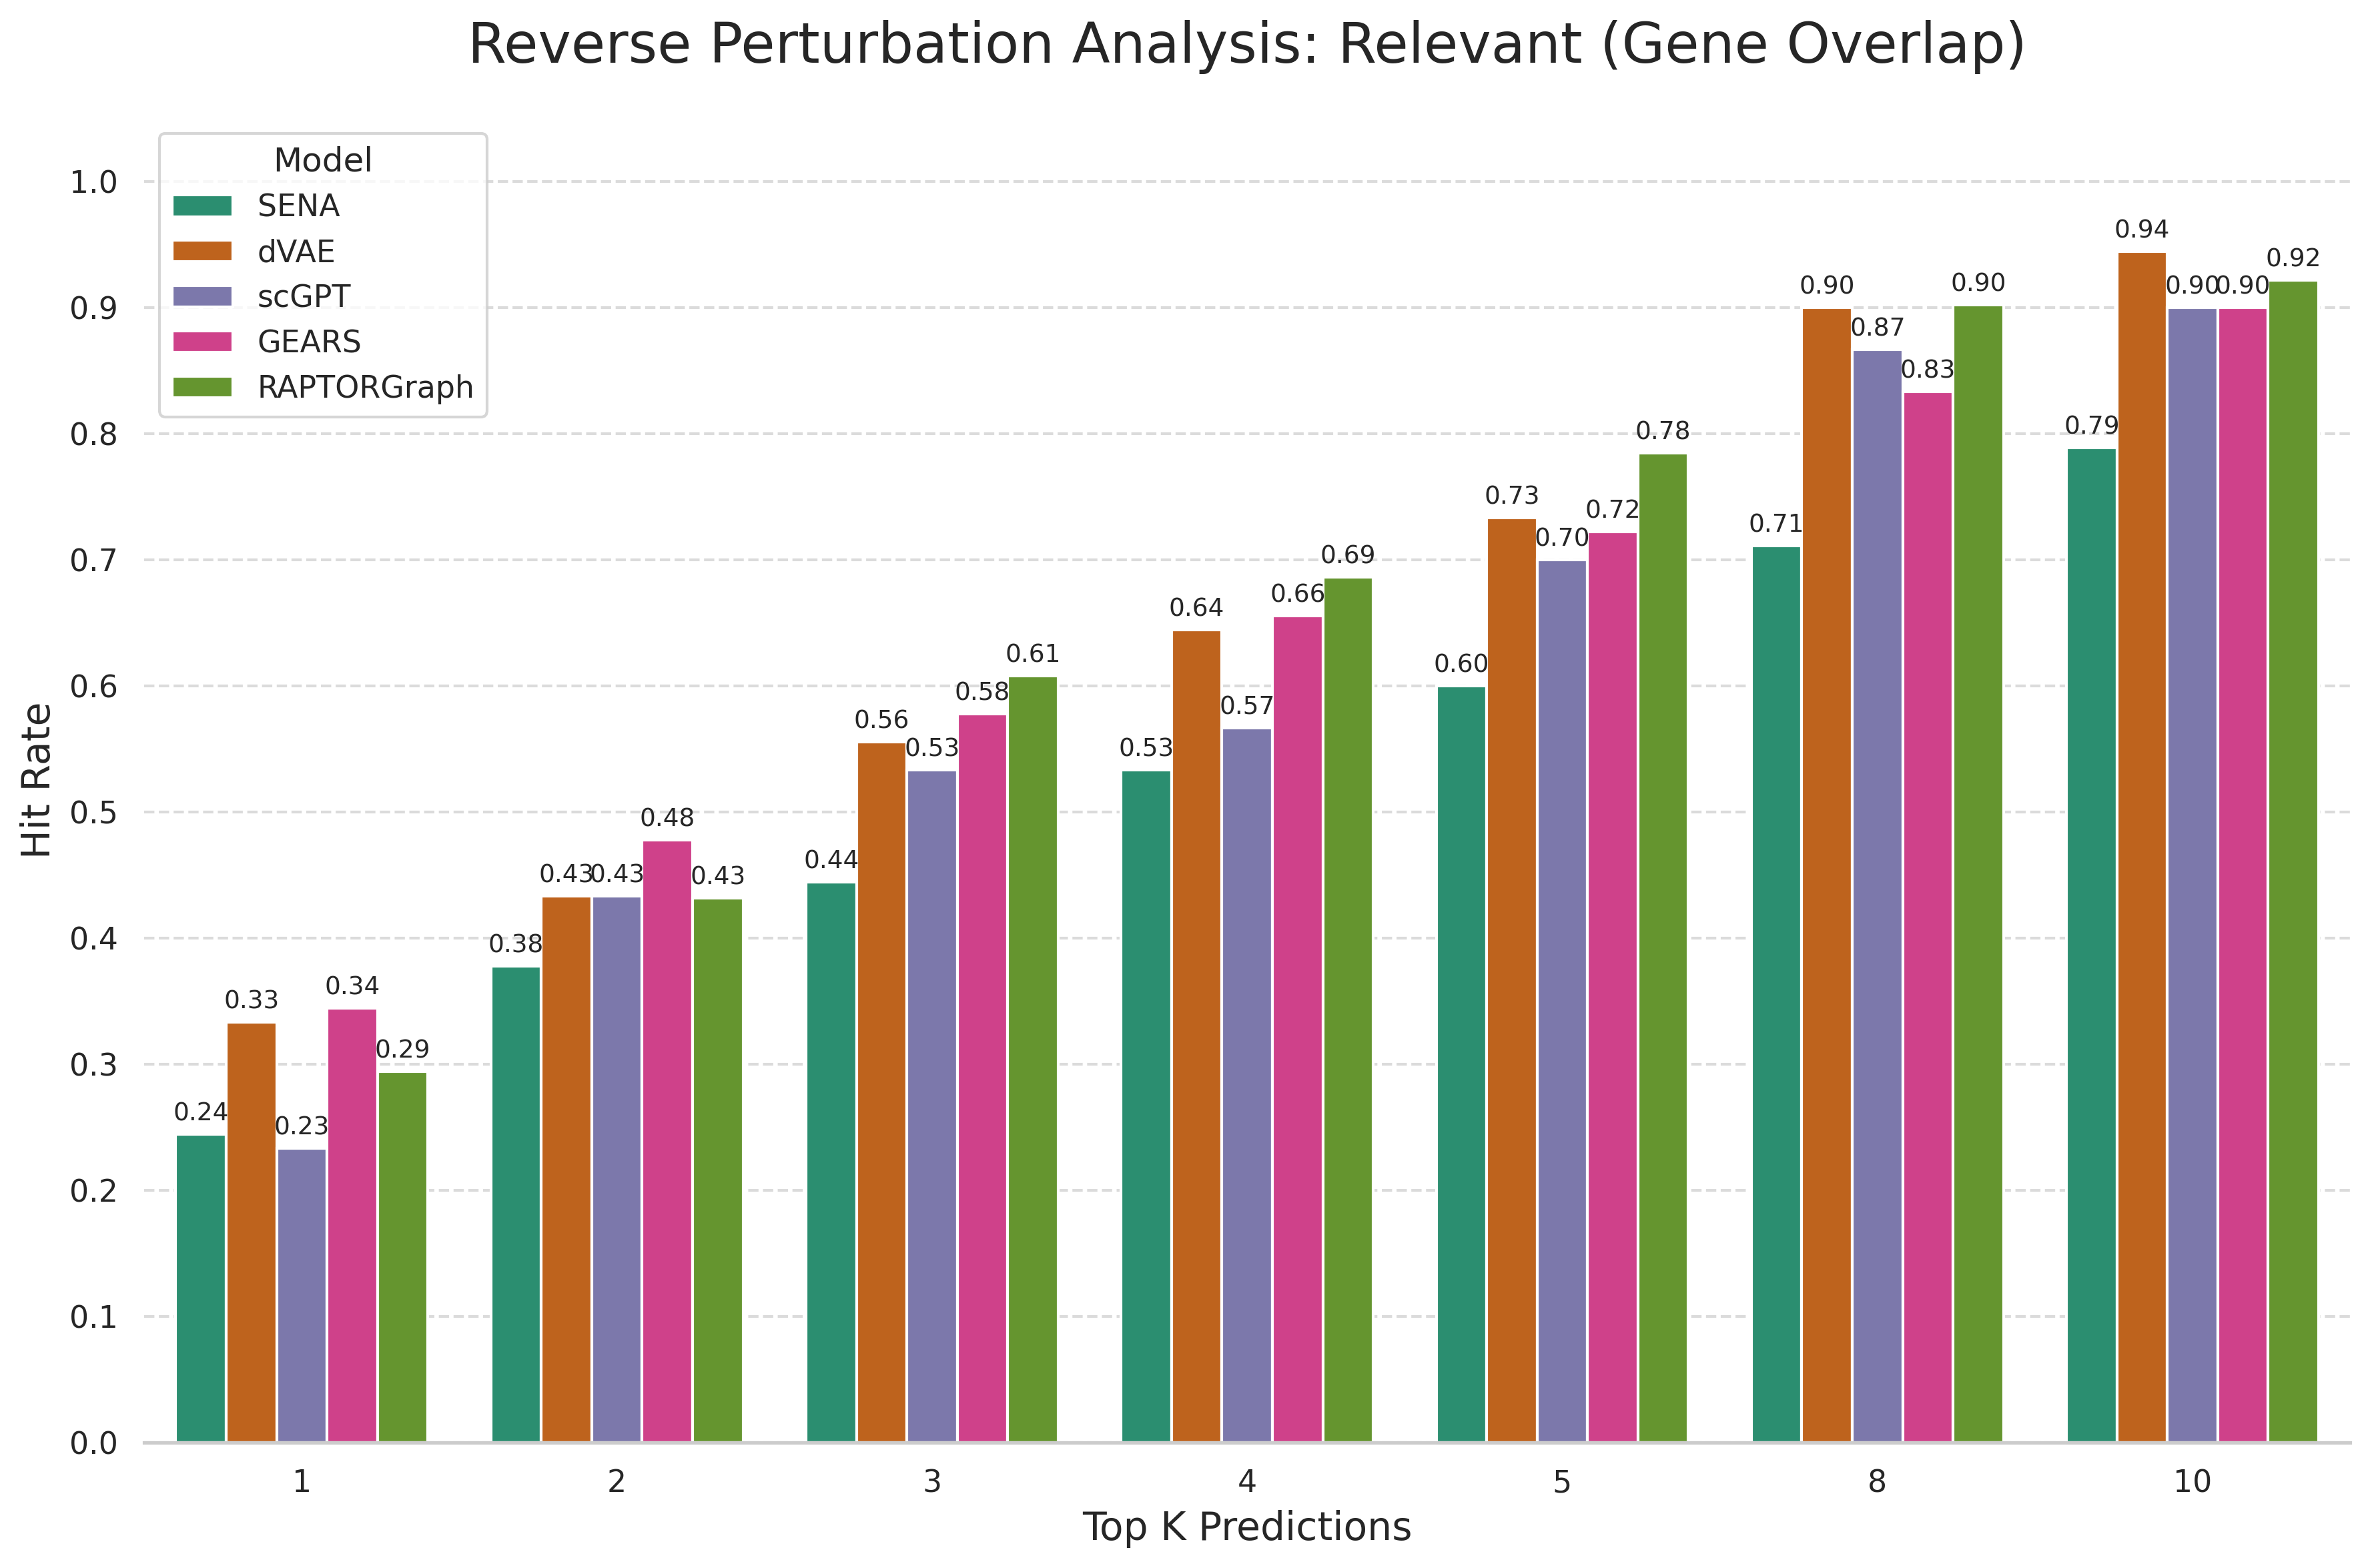
\includegraphics[width=0.98\linewidth]{gfx/results/hit_rate_at_k_relevant_gene_overlap.png}
    \caption{Hit Rate @ K (averaged over 3 runs).
    The metric measures the fraction of queries where at least one correct gene was identified in the top K predictions.
    Higher is better.}
    \label{fig:app:hit_rate_relevant}
    \vspace{-\baselineskip}
\end{wrapfigure}
While predicting genetic interactions demonstrates a model's forward predictive power, a more profound test is its ability to reverse-engineer the genetic cause of an observed phenotype.
To this end, we challenged a model to identify the specific genetic perturbation responsible for a given cellular gene expression profile.
The analysis was performed on a controlled combinatorial space of 20 transcription factors from the \citet{norman2019exploring} dataset.
For each model, we generated a database of predicted expression profiles for all possible double-gene perturbations within this subset.
We then used the ground truth mean expression profiles from experimentally observed double perturbations as queries, ranking the database entries by similarity to identify the most likely causal perturbation.

We first evaluated the models on the highly stringent task of identifying the exact causal gene combination, quantified by the Correct (Exact Match) Hit Rate @ K.
As shown in \cref{fig:app:hit_rate_exact}, all models achieve modest hit rates, underscoring the profound difficulty of this reverse-engineering challenge.

However, a more practical measure of a model's utility to guide experimental genetic perturbation designs is its ability to retrieve perturbations containing at least one of the correct genes. We thus evaluated each model's capacity to identify biologically influential genes using the Relevant (Gene Overlap) Hit Rate @ K (see \cref{fig:app:hit_rate_relevant} and \Cref{tab:hit_rate}).



\Gls{raptorgraph}  demonstrates exceptional performance, consistently ranking among the top models.
This highlights that while pinpointing exact higher-order interactions is an ongoing challenge, \gls{raptorgraph} is highly effective at identifying the key genetic players driving a cellular response, making it a highly valuable tool for hypothesis generation and experimental design.
\begin{table}[htb]
\centering
\caption{
    Hit Rate @ K (relevant) for the reverse perturbation task.
    The metric measures the fraction of queries where at least one correct gene was identified in the top K predictions.
    Higher values are better.
    \revised{Values are mean $\pm$ variance over 3 runs.}
}
\label{tab:hit_rate}
\vskip 0.15in
    \begin{center}
    \begin{small}
    \resizebox{\columnwidth}{!}{%
    \csvreader[
        separator=comma,
        tabular= lccccc,
        table head=\toprule $k$ & \gls{dvae} & SENA & GEARS & scGPT & \gls{raptorgraph} (ours)\\ \midrule,
        late after line=\\, 
        table foot=\bottomrule
    ]{results_files/hit_rate/hit_rate_at_k_summary_transposed.csv}{k=\k,SENA=\SENA,scGPT=\scGPT,dVAE=\dVAE,GEARS=\GEARS,RAPTORGraph=\RAPTORGraph}
    {\k & \dVAE & \SENA & \GEARS & \scGPT & \RAPTORGraph}
    }
    \end{small}
    \end{center}
\vskip -0.1in
\end{table}


\section{\revised{\gls{raptorgraph} learns biologically meaningful \cmps{}}}

\revised{To confirm that \gls{raptorgraph} learns biologically meaningful causal structures rather than arbitrary representations, we examined the functional identity of the \cmps{} using Gene Set Enrichment Analysis (GSEA).
For each \cmp{}, we identify the $N$ single-gene interventions that induce the greatest change in that meta-pathway.
Then, for every such ranked gene list, we perform a GSEA to identify significantly enriched biological processes (also known as pathways) within this set of $N$ genes, serving as transcriptional signatures for the causal meta-pathway. It is important to differentiate between the GSEA-derived pathways (which are well-described biological processes from known databases) and the causal meta-pathways (which are learned causal latent factors that are associated with single interventions). Thus, our goal here is to assess whether the learned causal meta-pathways encompass relevant and related biological processes.
For this evaluation, we use the ``Hallmark'' gene sets from the Human Molecular Signatures Database (MSigDB) database~\citep{liberzon_molecular_2015}.}
%We observed a robust alignment between the known biological roles of perturbed genes and the pathway enrichments of their corresponding \cmps{}.

\revised{The GSEA analysis reveals that \gls{raptorgraph} captures distinct and biologically accurate programs. \Cref{fig:app:pathway_heatmap_supp} visualizes the Normalized Enrichment Scores (NES) for the top enriched pathways across the learned factors. We highlight distinct biological programs captured by the model, verified against the known functions of their corresponding gene perturbations:}
%
\begin{enumerate}[leftmargin=*]
     \item \revised{\textbf{Differentiation-Induced Arrest:} The \cmp{} linked to \textit{EGR1} displays massive negative enrichment for ``E2F Targets'' and ``G2-M Checkpoint''.
    EGR1 is a known tumor suppressor in K562 leukemia cells that drives differentiation along the megakaryocytic lineage, a process that necessitates a complete exit from the cell cycle \citep{ma_emodin_2019}.
    \gls{raptorgraph} correctly identifies this potent anti-proliferative program.}
    \item \revised{\textbf{Stress-Induced Growth Arrest:} The \cmp{} linked to the AP-1 subunit \textit{JUN} shows strong negative enrichment for ``E2F Targets'' and ``G2-M Checkpoint''. While often associated with inflammation, c-Jun is a central stress-response mediator; in the context of K562 cells, its activation drives a termination of cell division required for stress adaptation or differentiation \citep{shaulian_ap-1_2002, shaulian_mammalian_2000}.}
    \item \revised{\textbf{p53-Like Tumor Suppression:} The \cmp{} associated with \textit{TP73} displays significant negative enrichment for ``G2-M Checkpoint''.
    \textit{TP73} is a functional homolog of \textit{TP53} (p53); its activation triggers downstream checkpoint signaling that arrests the cell cycle to prevent genomic instability \citep{kaghad_monoallelically_1997}.}
\end{enumerate}
%
\revised{
These findings confirm that the nodes in our learned DAG represent specific biological mechanisms and that the edges learned by the DAGMA module can be interpreted as causal regulatory links between these verified biological processes. A detailed description of the methodology is provided in \cref{app:metrics:gsea_setup}.
}
%
Detailed GSEA results and the associated enrichment heatmap are provided in \cref{app:extended_results:biological_validation}.